\chapter{Distribution protocol}

As introduced in Chapter~\ref{chap:intro}, there are two circumstances in software update,  software upgrade and 
software switch. The software upgrade happens when the application that is already running in the WSN needs to be 
changed for bug fix or adding new features. So in this case, there is one source node -- the sink, and multiple 
destination nodes in the network. However, The software switch happens in MA-WSNs, where multiple applications are 
already deployed in the network. Because some neighboring nodes may already have the wanted binary code in memory, the 
code distribution problem here is how to route the code image from sensors to sensors. In this case, there are multiple 
source nodes in the network, which is different from the software upgrade case. Because of this difference, I propose 
to use two different code distribution protocols for the two different cases.


\section{Broadcast based code distribution protocol (Deluge)}
While doing software upgrade, the upgrade patches are generated on the sink node using the proposed update-conscious 
compiler techniques to improve the code similarity with the older version of such application. Then the patch is 
generated in the script format as mentioned above.After the patches are generated on the sink node, the network 
protocol Deluge~\cite{deluge} is used to disseminate the scripts to the network. 

The protocol works as follows. 
First, the whole update script is divided into fixed size pages.
At the beginning, the states of nodes are set to {\it Maintain} state. 
Each sensor node keeps broadcasting the advertisement messages ({\it ADV}) periodically,
which contains the information of the application code that it has. 
When a sensor node {\it S} receives an advertisement, which indicates that the neighbor 
{\it N} has a newer version of the application in its memory or has finished downloading more pages, node S will send 
out a request message ({\it REQ})
to {\it N} to request for a page, and change its own state from {\it Maintain} to {\it Request}.
The state will be changed back when it receives all the packets in the requested page.
Node {\it N} will change state to {\it Transmit} when it receives the request message from
{\it S}. Then it will start sending all the packets of the requested page to node {\it S}.
After the code transmission is finished, the state will be changed back to {\it Maintain} state.
Figure~\ref{fdeluge} shows the advertise-request-data handshaking protocol used Deluge~\cite{deluge}.

\begin{figure}[htbp]
\centering
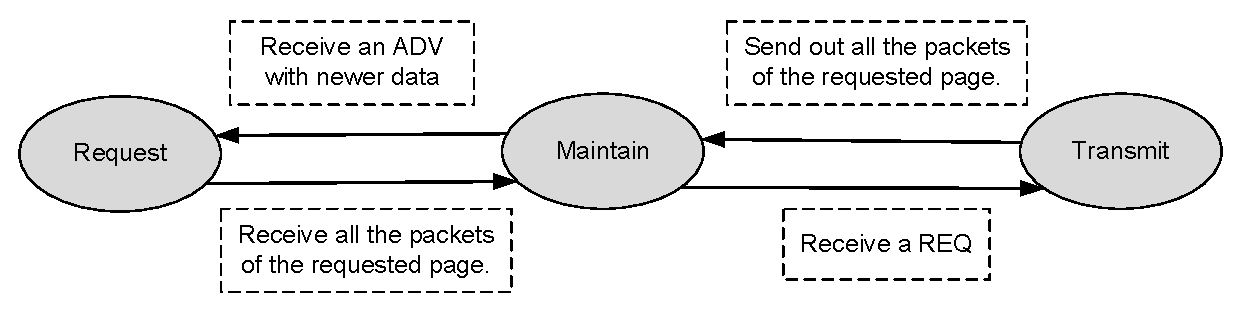
\includegraphics[width=4.2in]{figures/deluge.eps}
\caption{Advertise-request-data handshaking protocol in Deluge.}
\label{fdeluge}
\end{figure}

These packets may be
encrypted and/or authenticated for security protection~\cite{sluice,secDiss1}. The
packets may also be grouped so that when remote sensors receive groups
out of order, they are still able to perform updates independent of
the receiving order.


\section{Multicast-based code redistribution protocol (MCP)}
	
\subsection{The software switch problem in MA-WSNs}
	
While doing software switch, the problem is a little bit different. The following example shown in Figure~\ref{fnet} 
illustrates the protocol design challenges here. 
Three applications are distributed across different nodes in a network. The code distribution problem arises when there 
is a need to reprogram some nodes to run application {\it A}.

\begin{figure}[htbp]
\begin{center}
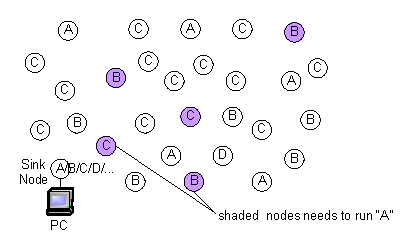
\includegraphics[width=3in]{figures/fnet.eps}
\caption{An example of software switch in a multi-application WSN (MA-WSN).}
\label{fnet}
\end{center}
\end{figure}

There are two existing approaches. A naive solution is to directly apply Deluge and disseminate application {\it A} 
from the sink to all sensors. After dissemination, the nodes that do not need {\it A} discard the code from their 
storage. The solution is clearly not a good choice due to unnecessary packets transmissions to the nodes that don't 
need it. The other solution is to let requesting nodes initiate code dissemination and fetch {\it A} from nearby 
sensors. Melete~\cite{melete} is such a protocol --- the nodes that need to run {\it A} broadcast their requests within 
a controlled range and discover the source nodes that have {\it A}. Sources then send back the requested data packets. 
However, as a stateless protocol, Melete does not record the source nodes and has to discover them repeatedly. When 
transmitting applications with multiple pages, multiple sources within the range may respond and thus create 
significant signal collision. 


\subsection{A multicast-based code redistribution protocol (MCP)}


I propose a multicast-based code redistribution protocol,  MCP, to solve the ``n to n'' code distribution problem in 
software switch. MCP employs a gossip-based source node discovery strategy. Each sensor summarizes the application 
information from overheard advertisement messages, and stores this information in a local application information table 
(AIT). Future dissemination requests are forwarded to nearby source nodes rather than flooding the network.
Different from the Deluge~\cite{deluge} scheme discussed above, the data messages are only multicast to the requesters, 
which avoids the unnecessary packet transmission in the network. With the guide of AIT, the request messages can be 
directly sent to the source nodes, which avoids the request message flooding in the network.  

An overview of this protocol is as follows.

\begin{itemize}
\item 
Sensors in MCP periodically broadcast {\it ADV} messages to advertise their knowledge about running applications in the 
network, which is similar to Deluge. Each sensor summarizes its overheard {\it ADV} messages in an {\em application 
information table (AIT)}. 

\item
To reprogram a subset of sensors, the sink floods a dissemination command that guides which sensors should switch to 
run application {\it A}. For example, a command ``[B$\rightarrow$A, p=0.25]'' indicates that the sensors whose active 
application is ``B'' should switch to ``A'' with a 25\% probability. That is 25\% of the nodes that are currently 
running application ``B'' will switch to ``A''.

\item
After receiving the command from the sink, each sensor identifies its dissemination role as one of the followings.  \\
(i)  a {\em source} if the sensor has the binary of application {\it A}; \\
(ii) a {\em requester} if the sensor does not have the binary of {\it A} but needs to switch to run {\it A}; or  \\
(iii) a {\em forwarder} if the sensor is neither a {\em source} nor a {\em requester}.

\item
A {\em requester} periodically sends out requests (i.e., {\it REQ} messages) to its closest source, until it acquires 
all the pages of application {\it A}. Instead of broadcast, the {\it REQ} messages are sent to the source via 
multicast. A requester resends the {\it REQ} message until it timeouts. It tries to request data from each source node 
several times before marking the node as a {\em temporary non-available} source.

\item 
A source node responds with the data (i.e., {\it Data} messages) that contain code fragments while a forwarder forwards 
both request and data packets. 
\end{itemize}

Similar to Melete and Deluge, MCP has three types of messages: an {\it ADV} message that advertises interesting 
applications; a {\it REQ} message that asks for packets of a particular page; and a {\it Data} message that contains 
one data packet (i.e, a piece of code segment).

\subsection{ADV message and application information table (AIT)}
In MCP, each sensor periodically broadcasts ADV messages, and summarizes the information of overheard ADV messages into 
a small application information table (AIT). Fig. \ref{fait} illustrates the algorithm.

Each {\it ADV} message contains the information of one application: (i) an application ID and version number; (ii) the 
number of pages of the application; (iii) the information of two closest source sensors --- the source ID and number of 
hops to the source (S, H); (iv) the CRC checksum. 
If a sensor has multiple known applications, it advertises them in a round-robin fashion. Note that a sensor may not 
have the code images of all its known applications. 

\begin{figure}[htbp]
\begin{center}
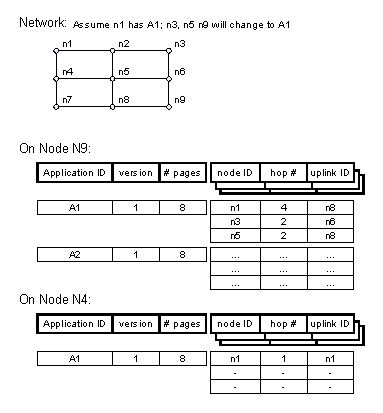
\includegraphics[width=4in]{figures/ftable.eps}
\caption{An example of the application information table (AIT).}
\label{fait}
\end{center}
\end{figure}




The AIT summarizes the overheard ADV messages. In addition to the application summary, AIT stores up to three closest 
source nodes for each known application, and the uplink sensor ID for each source, i.e., from which the source 
information was received.
The size of each application entry in the AIT is 12 bytes. Assume that the number of the applications running in the 
network is 10,
the AIT size will be only 120 bytes, which makes it fit perfectly in the program memory.

When an incoming ADV message contains new information, the corresponding entry in the AIT is updated. Assume a sensor 
S1 receives an ADV message from S2, and the message identifies two nearby sources (S3, H3) and (S4, H4) where H3 and H4 
indicate the number of hops from S2 to sources S3 and S4. If S1 already records the information of three sources (S5, 
H5, U5), (S6, H6, U6), and (S7, H7, U7), then it updates the AIT table according to the following rules. 

\begin{itemize}
\item
If one entry in AIT table records the previous message from the same uplink S2 and it refers to the same source, e.g. 
S5=S3 and U5=S2, then the information in the ADV message represents the up-to-date source information and replaces the 
old entry.

\item
If one entry in the AIT records a longer path to an advertised source, e.g. S5=S3, U5$\ne$S2, and H5$>$(H3+1), then the 
hop count and uplink node from the ADV message replace those in the AIT.

\item
If the advertised source cannot be found in the AIT, and there is an invalid entry in the table, then the new source is 
inserted into the table.

\item
If the ADV message advertises a closer source than one of those in the AIT table, then the closer source replaces the 
farthest source in the AIT. 

\end{itemize}

Each sensor advertises the application in the AIT in a round-robin fashion, and prioritizes the applications whose 
entries have been recently updated: (i)~the applications whose sources were recently updated are advertised before 
those that were not; (ii) in one round, the applications whose sources were recently updated are advertised three times 
while others are advertised once. In addition to normal ADV advertisement, an application is advertised if the sensor 
receives a broadcast request for that application, as we elaborate next.

\subsection{Request multicasting}
In MCP, a requester continues to send out request messages until it receives all pages of the target application. Given 
the target application, the requester searches the AIT for a closeby live source and constructs a REQ message as follows
\begin{center}
REQ = [S, H, pgNum, bv] \\
\end{center}
where S indicates the selected source node, H indicates the maximum number of hops that the message may travel, pgNum 
and bv indicate the current working page and the requested packets in the page. If the AIT records more than one source 
node, then the requester selects the closest live source and sets H to h+$\delta$ where h is the number of hops to S 
(recorded in the AIT), and $\delta$ is the hop count slack allowed in the dissemination. 
Fig. \ref{fgrad} illustrates the involved nodes when h=2 and $\delta$=1. These nodes routed through a gradient-based 
region~\cite{groute} to the source. 

\begin{figure}[htbp]
\begin{center}

\includegraphics[width=1.5in]{figures/fgrad.eps}
\caption[Gradient-based request routing.]{Gradient-based request routing. R and S are requester and source nodes 
respectively; h=2; $\delta$=1.}
\label{fgrad}
\end{center}
\end{figure}

A requester continues sending the REQ messages when it can not finish the page before timeout. After several tries, it 
marks the source that it tried
to reach as an {\em unreachable} source. The number of tries varies based on the distance to the source. 

If the AIT does not record any nearby source, then the requester sets~S to be {\em null}, indicating the REQ message is 
sent to all neighbors. After receiving a broadcast request, an idle forwarder forwards the request unless the message 
has travelled the maximum number of hops; an idle source node always responds with requested packets.

%If the sensor records a local source in its AIT, however the corresponding uplink of the AIT entry is not the node 
from which the request was %received, the sensor advertises the source information. 

Since each requester sends out REQ messages independently, different requesters may work on different pages. MCP allows 
node preemption. If a REQ message asking for page $x$ reaches a working node who is currently working on page $y$, and 
$x+1 < y$, then the node quits the current state and switches to serve the request. If the node is a forwarder, then it 
forwards the request; if the node is a requester or a source, then it must have the requested page and thus will 
respond with the requested packets. The node enters the idle state after serving the request.

\subsection{Caching}
During code dissemination, some requesters or forwarders, while working on the current page, may overhear packets from 
pages with larger indices. As code pages are requested strictly in increasing order, a requester will work on 
large-number-indexed pages, and a forwarder has a high possibility to receive requests for these pages. 

To improve transmission efficiency, sensors in MCP buffer such packets in their data memory. The space that can be 
dedicated to caching on a wireless sensor is usually very limited. While it is possible to exploit external flash for 
caching, accessing external flash is slow and writing it has to be performed in 256-byte blocks, which complicates the 
design and wastes the energy. 

Caching on a requester is straightforward as the sensor always caches the next several pages in addition to the current 
working page. However, it is slightly more complicated on a forwarder node as it gets requests from different 
requesters that work on different pages and may suffer from thrashing if it takes turns to serves these requests. In 
MCP, a forwarder gives priority to pages with smaller indices. We set a timer for the cached page and clear the page 
after serving a request or timeout.


\section{Simultaneous code dissemination}
As shown in~\cite{melete}, different applications in a MA-WSN
usually share some code segments. For example, two applications
may be designed for sensing and processing two different
events like wildfire and animal mitigation. While the
data processing components are different, the routing code
could be similar. If one application has already been installed
on some sensors, then at the time when a remote sensor
wants to load the other application, it is energy efficient
to fetch the common code from these peer sensors instead of
the sink. 

Fetching code from peer sensors exhibits two advantages:
(i) remote requesting sensors (i.e. the sensors that
need to switch their running application to the new one) can
start early and fetch the code in parallel without waiting for
the progressive code dissemination from the sink. (ii) since
only a subset of sensors get involved in dissemination, the
message overhead can be greatly reduced. Without losing
generality, we assume $A$ and $B$ share $S_{ab}$ common packets
while $A$ and $C$ do not share any packet. When a sensor
needs to switch to run application $A$, it fetches shared code
from nodes that have $B$ and the rest of the code from the
sink.

\begin{figure}[htbp]
\begin{center}
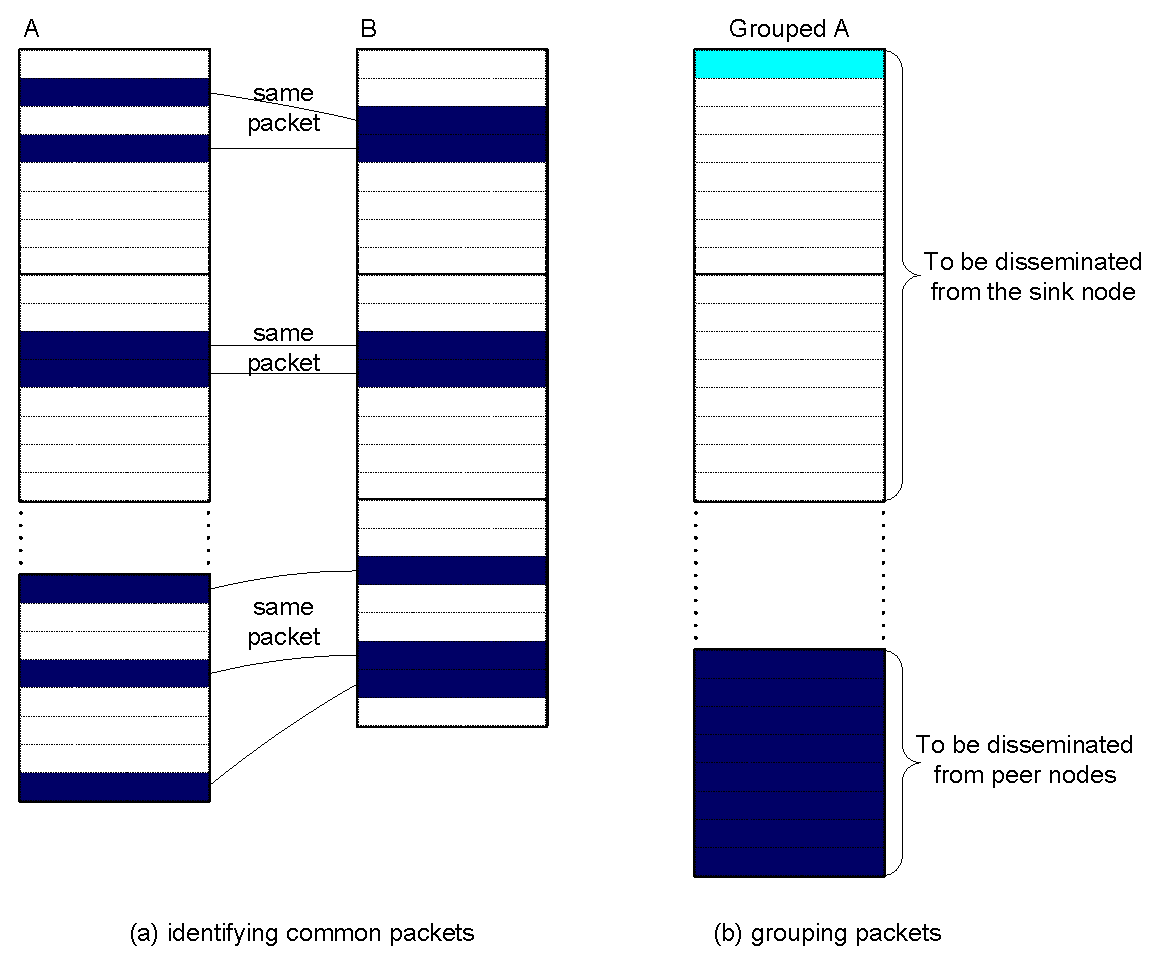
\includegraphics[width=4.5in]{figures/common.eps}
\caption{Simultaneous code dissemination.}
\vspace{-0.3in}
\label{common}
\end{center}
\end{figure}

The basic dissemination unit in MA-WSN is a packet
that contains 23 bytes payload, similar as that in the default
multi-hop dissemination protocol Deluge~\cite{deluge} in TinyOS. To
enable code dissemination of two types of packets, the code
segments needs to be reorganized, as shown in Fig~\ref{common}. Given
the above application $A$ to be disseminated, we first divide
it into a sequence of code packets, and mark all packets
that are shared with $B$. We compare at the packet level in
this paper while techniques have been proposed to compare
two applications and generate difference at different levels
~\cite{melete,ucc} After marking the code, we group packets based
on if they are marked or not, and add two bit vectors (one
vector per application and one bit per packet) to guide the
code reorganization. The bit vector for application $A$ (or
$B$) indicates the locations of marked packets in application
$A$(or $B$). For example, a bit vector 